\documentclass[a4paper]{article}

\usepackage[utf8]{inputenc}
\usepackage[T1]{fontenc}
\usepackage[french]{babel}
\usepackage{listings}
\usepackage{graphicx}
\usepackage{chngpage}

\begin{document}
\begin{adjustwidth}{-2cm}{-2cm}
\title{Serveur de temp NTP}
\author{Rémy De Poorter}
\date{2022}
\maketitle
\newpage

\tableofcontents
\newpage

\section{Introduction}
Sur un serveur beaucoup de programmes utilisent l’heure système. Par exemple l'on peut enregistrer l’heure des logs, la connexion d’un utilisateur, l’heure d’une commande sur un site internet. Il faut donc avoir une mesure du temps précise pour permettre la communication entre plusieurs machines. Celles-ci vont utiliser une même mesure du temps pour synchroniser leurs actions
\newline
\newline
L’on peut configurer manuellement l’heure d’une machine mais ce n’est pas assez précis. C’est pourquoi le protocole NTP (Network Time Protocole) qui est l’un des plus vieux protocoles, est apparu en 1985.

 \newpage
\section{Architecture}
NTP permet de synchroniser l’heure des différents systèmes à travers un réseau IP. Les clients vont synchroniser leur horloge avec le serveur et chaque serveur se synchronise avec lui-même ainsi que d’autres serveurs. Ce réseau forme donc des couches appelées strata (stratum au singulier). Le plus haut niveau est 0 ce seront des matériels spécialisé couplé avec des horloges atomique. Chaque niveau possède un temps fiable et permet de répartir la demande de temps entre les différents serveurs et d’éviter que l’un soit surchargé.
\newline
\newline
Une horloge atomique est une horloge qui définit un temps en analysant la fréquence du rayonnement électromagnétique émis par un électron lors du passage d’un niveau d’énergie à un autre. Cela permet d’avoir un temps exact et très stable.

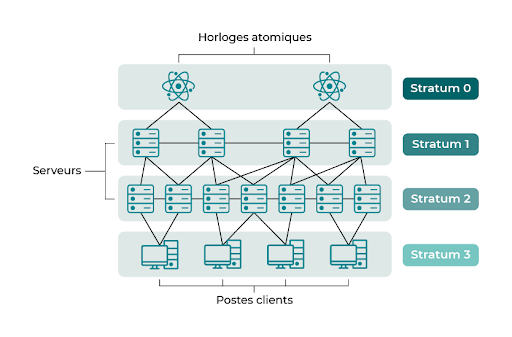
\includegraphics[scale=0.6]{picture/2.png} 
\newline
Beaucoup d'organisations gèrent leurs propres serveurs de temps. Certaines n’autorisent qu’une utilisation interne tandis que d'autres autorisent une utilisation publique. Un des plus grands clusters de serveur NTP publics est appelé pool.ntp.org. C’est celui-la qui est configuré par défaut dans la plupart des distributions linux.

\newpage
\section{Faut-il obligatoirement configurer son propre serveur ?}
 Il est possible d’utiliser le serveur NTP mondial qui est présent par défaut pour synchroniser l’horloge des serveurs mais lorsque le réseau grandit il est intéressant d’avoir son propre serveur NTP car
\begin{itemize}
    \item La synchronisation entre les serveurs du réseau de l’entreprise sera meilleure avec seulement quelques millisecondes les un des autres..
    \item Le trafic dû aux synchronisations vers internet sera réduit. Car la définition de l’heure se fera localement et il ne faudra donc pas sortir du réseau local.
    \item Si un problème technique comme une coupure de courant survient les serveurs restent synchronisés entre eux.
    \item Cela permet aussi de ne pas dépendre du réseau mondial NTP.
\end{itemize} 
Attention, NTP ne s'occupe pas de tout, en effet l’heure de référence fournie est UTC (temps universel coordonné). Le système d’exploitation aura la tâche de gérer le changement d’heure et les fuseaux horaires en fonction de la position de la machine cliente.
Les messages NTP ne sont pas cryptés par NTP et peuvent donc circuler librement sur le réseau. Il est possible de les crypter mais cela va alourdir les paquets à transférer et n’a pas forcément d'intérêt à être sécurisé.
\newline
\newline
Un serveur NTP est sensible aux attaques de DDOS. Par exemple, un hackeur peut utiliser de fausses adresses IP d'expéditeur et envoyer des paquets au serveur. L’adresse du système embarqué est choisie comme adresse d’expéditeur. Le serveur renvoie sa réponse à l’expéditeur supposé, qui sera la victime. En faisant cela à grande échelle, le système ciblé pourra être surchargé.


 
 \newpage
\section{Les meilleures pratiques}
Utiliser des ntp publics pour les hôtes externes :
\newline
Si l’entreprise utilise des services, développe des capacités ou d’autres plates-formes intégrées destinées à être déployées hors de l’entreprise, il est envisageable de demander un serveur NTP public à partir du pool de serveur disponible. Il faudrait alors configurer une hiérarchie pour définir les serveurs utilisés pour se synchroniser pour éviter la concurrence d’accès entre le serveur ntp public et celui de l’entreprise.
\newline

Configurer son propre serveur ntp interne :
\newline
Il est possible d’acheter des appliances NTP Stratum 1 ou 0 à utiliser en interne, ou de mettre en place son propre serveur NTP pour un faible coût.
\newline

Standardiser sur le temps UTC :
\newline
Normaliser tous les appareils au système universel de temps UTC permet de simplifier la corrélation des journaux entre l’organisation et les parties externes, quel que soit le fuseau horaire utilisé par l’appareil.
\newline

Sécuriser le service de réseau de temps :
\newline
Il est recommandé de restreindre les commandes utilisables sur le serveur stratum, de ne pas autoriser les requêtes publiques des serveurs de strate et donc d’autoriser uniquement les réseaux connus.
\newline

Cryptage :
\newline
Il existe des services de cryptage associés à NTP mais le cryptage n’est pas toujours nécessaire. L’entreprise en a-t- elle vraiment besoin et à quel niveau de complexité ? Plus un échange est crypté, plus il sera sécurisé mais consomme aussi davantage de ressources et apporte avec lui des sources de problèmes potentiels supplémentaires.
\newline

Lois de Segal :
\newline
Avoir plusieurs sources de temps permet de maintenir une heure précise même en cas de panne de l’un des serveurs.
La loi de ségal dit que si on a deux serveur d’horodatage avec une heure différente on ne peut pas savoir la quelle est la plus précise. C’est pourquoi il est conseillé d’avoir au moins 3 serveurs stratum 0 ou stratum 1 et de les utiliser comme maîtres principaux. Il est aussi conseillé de répartir géographiquement les différents serveurs.
\newline

Gérer le nombre de clients :
\newline
En cas de forte utilisation des serveurs de temps, l’on peut ajouter des stratum secondaire pour augmenter la bande passante et réduire la charge de travail des serveurs principaux.
\newline

Rester à jour.
\newline
Il est conseillé de faire les mises à jour du serveur de temps pour combler les failles. Et donc être mieux protéger des attaques réseau.

 \newpage
\section{Mise en place}
\subsection {Procédure pour modifier manuellement l'heure du sytème}
\noindent Afficher l’heure avec systemd :
\begin{lstlisting}[language=bash]
  sudo timedatectl
\end{lstlisting}
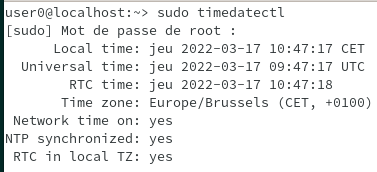
\includegraphics[scale=0.6]{picture/3.png} \\

\noindent Définir l’heure au format année mois jour heure minute seconde :
\begin{lstlisting}[language=bash]
  sudo timedatectl set-time "2015-11-20 16:14:50"
\end{lstlisting}

\noindent Afficher les fuseau horaires disponibles avec un filtre :
\begin{lstlisting}[language=bash]
  sudo timedatectl list-timezones | grep Brussels
\end{lstlisting}

\noindent Définir le fuseau horaire :
\begin{lstlisting}[language=bash]
  sudo timedatectl set-timezone | Europe/Brussels
\end{lstlisting}

\noindent Voir la synchronisation de l'heure :
\begin{lstlisting}[language=bash]
  sudo systemctl status systemd-timesyncd.service
\end{lstlisting}
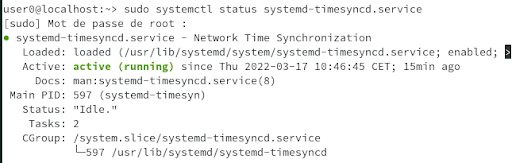
\includegraphics[scale=0.7]{picture/4.png} 
\newpage
\subsection {Procédure pour mettre en place un serveur utilisant le pool de serveur ntp}

Configurer le serveur\\ \\
\noindent connaitre l'adresse ip du serveur :
\begin{lstlisting}[language=bash]
 sudo ip a
\end{lstlisting}
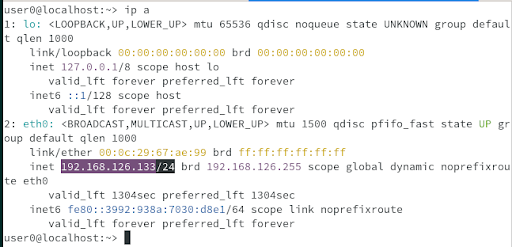
\includegraphics[scale=0.7]{picture/5.png} \\

\noindent Sur OpenSuse le serveur NTP par défaut s'appelle chrony, l'installer si ce n'est pas déjà fait à l'aide de :
\begin{lstlisting}[language=bash]
 sudo zypper install chrony
\end{lstlisting}
\newpage
\noindent Pour configurer chrony, il faut éditer le fichier de configuration de celui-ci :
\begin{lstlisting}[language=bash]
 sudo nano /etc/chrony.conf
\end{lstlisting}
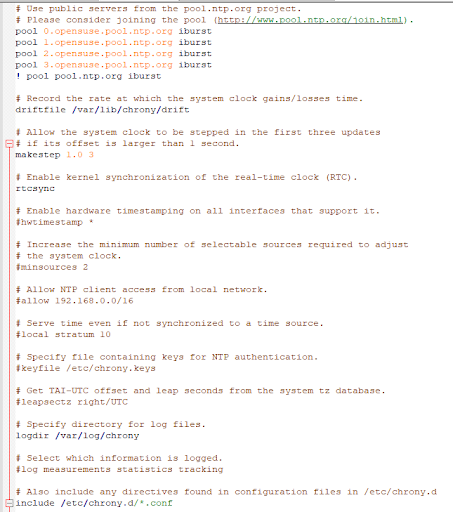
\includegraphics[scale=0.8]{picture/6.png} 

pool définit les serveurs utilisés pour se synchroniser par défaut c’est le site de opensuse. \newline

driftfile est le fichier dans lequel chrony va noter la différence de temps entre l’horloge locale et celle des serveurs de référence. \newline

rtcsync informera le noyau que l'horloge système est synchronisée et que le noyau mettra à jour l'horloge RTC toutes les 11 minutes. Donc commenter rtcsync

Par défaut chrony n’autorise pas les clients à se synchroniser avec notre serveur, il faut donc les autoriser en ajoutant la ligne suivante contenant le réseau du serveur avec
allow 192.168.0.0/16\newline

Ajouter un stratum local qui sera utilisé en cas de non connexion au serveur publics. \newline
local stratum 10 \newline
ensuite quitter en enregistrant les modifications.

\noindent Configurer le démarrage automatique de chrony avec le système :
\begin{lstlisting}[language=bash]
sudo systemctl enable chronyd
\end{lstlisting}

\noindent Démarrer le serveur :
\begin{lstlisting}[language=bash]
sudo systemctl start chronyd
\end{lstlisting}

Pour gérer le serveur chrony on utilise l’interface en ligne de commande chronyc\newline
\noindent afficher la liste des serveur ntp auquel le nôtre est synchronisé :
\begin{lstlisting}[language=bash]
sudo cronyc sources
\end{lstlisting}
* pour le serveur utilisé comme référence\newline
+ pour les serveur qui servent à calculer une moyenne de temps\newline
- pour les serveurs actuellement non utilisés.\newline \newline
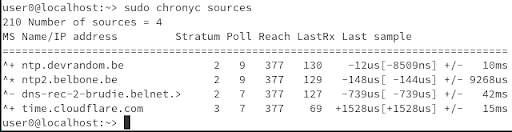
\includegraphics[scale=0.7]{picture/7.png} \newline

Configurer le client
\noindent éditer le fichier de configuration :
\begin{lstlisting}[language=bash]
sudo nano /etc/systemd/timesyncd.conf
\end{lstlisting}
ajouter l'ip du serveur \newline \newline
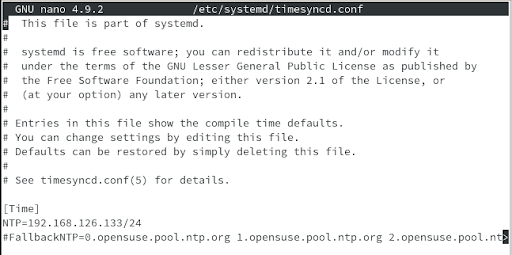
\includegraphics[scale=0.8]{picture/8.png} 
\newpage
\noindent redémarrer systemd :
\begin{lstlisting}[language=bash]
sudo systemctl restart systemd-timesyncd
\end{lstlisting}

\noindent redémarrer le chronyd :
\begin{lstlisting}[language=bash]
sudo systemctl restart chronyd
\end{lstlisting}

\noindent Afficher les sources utilisées par chrony :
\begin{lstlisting}[language=bash]
 chronyc sources
\end{lstlisting}
L'étoile correspond au serveur utilisé \newline \newline
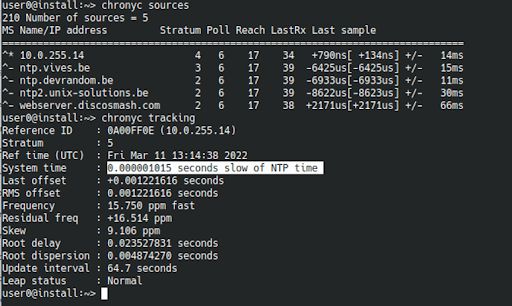
\includegraphics[scale=0.8]{picture/9.png} 

 \newpage
\subsection {Procédure pour créer un serveur ntp sans utiliser de pool public}
\noindent Pour le serveur suivre la procédure précédente mais changer ceci dans le fichier de configuration de chrony
\begin{lstlisting}[language=bash]
 sudo nano /etc/crony.conf
\end{lstlisting}
commenter les pools originaux car on en a plus besoin \newline
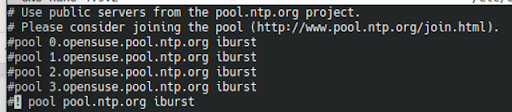
\includegraphics[scale=0.8]{picture/10.png} \newline
définir un stratum local
local stratum 10
allow 10.0.255.0/24

Pour le client ajouter comme source l’ip de notre serveur \newline
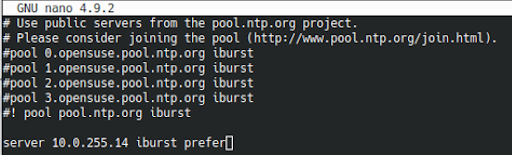
\includegraphics[scale=0.8]{picture/11.png} \newline

\noindent Redémarrer chronyd
\begin{lstlisting}[language=bash]
 sudo systemctl restart chronyd
\end{lstlisting}

 \newpage
\section {Procédure pour planifier une tâche avec cron.}
\noindent autoriser l'utilisateur à exécuter la tâche :
\begin{lstlisting}[language=bash]
 sudo nano /etc/cron.allow
 et y ajouter l'utilisateur (user0)
\end{lstlisting}

\noindent ajouter une tâche :
\begin{lstlisting}[language=bash]
 sudo crontab -e
\end{lstlisting}
ajouter les paramètres de temps ainsi que la commande à exécuter 
minute (1 à 60)
heure (1 à 24)
jours (1 à 31)
mois (1 à 12 ou leur libellé anglais jan, feb, mar)
jour (1 à 7 ou leur libellé anglais mon, tue, wed)
commande à lancer
une * est utilisée si on ne renseigne rien
*/1 veut dire que on lance la commande toutes les minutes si on avait seulement mis 1 alors la commande s'exécutera à chaque première minute de chaque heure (00h01, 01h01, 02h01, …)

 */1 * * * * echo “coucou” >> remy.txt


 \newpage
 \section{Alternative a NTP le SNTP}
 Une version simplifiée du protocole NTP est développée en parallèle. Elle s’appelle SNTP pour Simple Network Time Protocole. Elle est destinée à des réseaux ou la précision à la seconde suffit. C’est une version qui allège avec des algorithmes avec un traitement de paquets plus léger. Il est utilisé pour les systèmes embarqués où la capacité de calculs est très limitée. Cette implémentation du temps plus simple dialogue quand même avec des serveurs NTP standards. SNTP doit donc être utilisé que quand c’est nécessaire pour ne pas perturbé et fausser le réseau NTP. Il est également recommandé de n’utiliser SNTP que sur des systèmes clients.
 \newpage
 \section{ Planificateur de tâche CRON}
Cron est un programme qui va exécuter automatiquement des tâches à une date et une heure spécifiées (le vendredi 13 janvier 2022) ou selon un cycle (tous les ans).
Cron est aussi appelé le planificateur de tâche ou gestionnaire de tâche planifiées.
Les tâches sont définies dans le fichier /etc/crontab. Elles s'exécutent avec les droits de root sans demander le mot de passe.
Pour son utilisation voir procédures.

 \newpage
 \section{Conclusion}
 Le protocole NTP est très utilisé à travers le monde pour la synchronisation des machines.
Son succès est lié à sa facilité de mise en place avec plus de 20 ans d'expérience et de recherches il est donc très fiable. Les réseaux NTP ont révolutionné les méthodes de traitement des paiements, la sécurité en ligne en évitant que le client soit réglé à une heure différente de celle du serveur. On pourrait imaginer une prochaine version du protocole permettant encore plus de fiabilité et de précision pour déterminer le temps même en attendant la version actuellement utilisée en fait déjà un protocole incontournable.

\newpage
 \section{Bibliographie}
\begin{thebibliography}{99}

\bibitem{pa}  https://doc.opensuse.org/documentation/leap/archive/15.0/reference/html/book.opensuse.reference/cha.ntp.html

\bibitem{pa} https://chrony.tuxfamily.org/index.html

\bibitem{pa} https://doc.ubuntu-fr.org/ntp

\bibitem{pa} https://ubuntu.com/server/docs/network-ntp

\bibitem{pa} https://www.pool.ntp.org/zone/be

\bibitem{pa} https://chrony.tuxfamily.org/examples.html

\bibitem{pa} https://help.uis.cam.ac.uk/service/network-services/network-time-protocol-ntp/details-of-the-network-time-protocol-service

\bibitem{pa} https://insights.sei.cmu.edu/blog/best-practices-for-ntp-services/

\bibitem{pa} https://services.renater.fr/ntp/article/presentation\_ntp\_article

\bibitem{pa} https://www.cisco.com/c/fr\_ca/support/docs/availability/high-availability/19643-ntpm.html

\bibitem{pa} http://www.audentia-gestion.fr/cisco/pdf/1094258\_ntpm.pdf

\bibitem{pa} http://www.audentia-gestion.fr/cisco/pdf/1094258\_ntpm.pdf

\bibitem{pa} https://docs.microsoft.com/fr-fr/windows-server/networking/windows-time-service/how-the-windows-time-service-works

\bibitem{pa} https://en.opensuse.org/SDB:Cron

\end{thebibliography}

 \newpage
\section{Annexes}
Les commandes \newline

\noindent Affiche les informations sur l’heure de votre système :
\begin{lstlisting}[language=bash]
  timedatectl
\end{lstlisting}

\noindent Installer le logiciel chrony comme serveur ntp :
\begin{lstlisting}[language=bash]
  sudo zypper install chrony
\end{lstlisting}

\noindent Afficher l'adresse ip de la machine :
\begin{lstlisting}[language=bash]
  ip a
\end{lstlisting}

\noindent Éditer le fichier de configuration de chrony :
\begin{lstlisting}[language=bash]
  sudo nano /etc/chrony.conf
\end{lstlisting}

\noindent Lancer chrony au démarrage :
\begin{lstlisting}[language=bash]
  sudo systemctl enable chronyd
\end{lstlisting}

\noindent Démarrer ou redémarrer chrony :
\begin{lstlisting}[language=bash]
  sudo systemctl start chronyd
\end{lstlisting}

\noindent Vérifier le statut de chronyd :
\begin{lstlisting}[language=bash]
  systemctl status chronyd
\end{lstlisting}

\noindent Désactiver la synchronisation ntp gérer par systemd :
\begin{lstlisting}[language=bash]
  sudo timedatectl set-ntp false
\end{lstlisting}

\noindent Vérifier les sources utilisées par chrony :
\begin{lstlisting}[language=bash]
  sudo chronyc sources
\end{lstlisting}

\noindent Éditer le fichier de configuration de timesyncd :
\begin{lstlisting}[language=bash]
  sudo nano /etc/systemd/timesyncd.conf
\end{lstlisting}

\noindent (Re)Démarrer le service systemd :
\begin{lstlisting}[language=bash]
  sudo systemctl restart systemd-timesyncd
\end{lstlisting}

\noindent Vérifier le statut de systemde :
\begin{lstlisting}[language=bash]
  sudo systemctl status systemd-timesyncd
\end{lstlisting}

\noindent Désactiver le lancement automatique de chrony au démarrage du système :
\begin{lstlisting}[language=bash]
  sudo systemctl disable chrony
\end{lstlisting}

\noindent Stop chrony :
\begin{lstlisting}[language=bash]
 sudo systemctl stop chrony
\end{lstlisting}

\noindent Définir l’heure au format année mois jour heure minute seconde:
\begin{lstlisting}
sudo timedatectl set-time "2015-11-20 16:14:50"
\end{lstlisting}
\newpage
\noindent Pour afficher les fuseau horaires disponibles :
\begin{lstlisting}[language=bash]
 sudo timedatectl list-timezones
\end{lstlisting}

\noindent Pour afficher les fuseau horaires disponibles à l'aide d’un filtre :
\begin{lstlisting}[language=bash]
 sudo timedatectl list-timezones | grep Kiev
\end{lstlisting}

\noindent Autoriser un user à exécuter des tâches programmées :
\begin{lstlisting}[language=bash]
 sudo nano /etc/cron.allow
 et y ajouter l'utilisateur (user0)
\end{lstlisting}

\noindent Interdire à un user à exécuter des tâches programmées :
\begin{lstlisting}[language=bash]
 sudo nano /etc/cron.deny
 et y ajouter l'utilisateur (user0)
\end{lstlisting}

\noindent Pour définir une tâche nous allons éditer le fichier :
\begin{lstlisting}[language=bash]
 sudo crontab -e
\end{lstlisting}
ensuite l’on défini le moment ou la commande va être exécutée :
minute (1 à 60)
heure (1 à 24)
jours (1 à 31)
mois (1 à 12 ou leur libellé anglais jan, feb, mar)
jour (1 à 7 ou leur libellé anglais mon, tue, wed)
commande à lancer
une * est utilisée si on ne renseigne rien
*/1 veut dire que on lance la commande toutes les minutes si on avait seulement mis 1 alors la commande s'exécutera à chaque première minute de chaque heure (00h01, 01h01, 02h01, …)
\newline \newline
Ce qui donne par exemple pour écrire coucou toutes les minutes dans le fichier remy.txt
*/1 * * * * echo “coucou” >> remy.txt
\newline \newline
\noindent Pour voir qu’elle s’est bien enregistrée on peut afficher la liste des tâche :
\begin{lstlisting}[language=bash]
 sudo crontab -l
\end{lstlisting}

\newpage
\section{Vocabulaire}
CRON \newline
Est un planificateur de tâche\newline

Chrony\newline
Est une implémentation versatile (qui change facilement) du protocole NTP.\newline

Chronyd\newline
Est un démon exécuter dans l’espace utilisateur\newline

Chronyc\newline
Est un outil en ligne de commande pour gérer chronyd\newline

BURST et IBURST\newline
Ils permettent de calibrer initialement et rapidement une horloge système.\newline
Burst envoie des paquets toutes les 2 secondes et IBURST toutes les 16 secondes pour synchroniser les horloges.\newline

BURST envoie une rafale de 8 paquets lorsque le serveur est accessible et est utilisé afin de mesurer avec précision la gigue.\newline

IBURST envoie lui aussi une rafale de 8 paquets mais dans ce cas si le serveur est inaccessible et raccourci les délais jusqu'à la première synchronisation. Spécifier IBURST permet donc d’avoir une synchronisation d’horloge plus rapide même si ce mode est considéré comme agressif envers certains serveur NTP publics car si le serveur ne répond pas le mode IBURST continue d'envoyer des requêtes fréquentes jusqu'à ce que le serveur réponde et que la synchronisation de l’heure démarre.\newline

La gigue\newline
Ce nombre est une valeur absolue en millisecondes, indiquant l'écart quadratique moyen de vos décalages.\newline

Driftfile\newline
Il est utilisé pour stocker le décalage de fréquence entre l'horloge système locale et celle de  fréquence requise pour rester synchronisée avec l'heure UTC. Le fichier de dérive est lu pendant le démarrage système et sa valeur est utilisée pour corriger la source horaire.  Utiliser ce fichier de dérive réduit le temps nécessaire pour atteindre une heure stable et précise. La valeur est calculée et le fichier est remplacé une fois par heure par ntpd.Le fichier de dérive est remplacé plutôt que simplement mis à jour c’est pourquoi ntpd possède l’autorisation d’écriture sur ce fichier.
\newline

RTC (Real Time Clock)\newline
Horloge de temps réel, l’horloge système.\newline
\newpage
RTCSYNC\newline
rtcsync informera le noyau que l'horloge système est synchronisée et donc le noyau mettra à jour l'horloge RTC toutes les 11 minutes.
Si aucun rtcfile ou rtcsync n'est dans la configuration, chronyd ne se souciera pas
du tout du RTC. Il ne suivra pas son décalage de fréquence par rapport à l'
heure système et ne corrigera pas la dérive avec l'option -s, ou ne demandera pas au
noyau de le synchroniser. Si le RTC dérive, l'heure initiale de démarrage
sera erronée.

\pagenumbering{arabic}
\end{adjustwidth}
\end{document}